% !TeX program = xelatex
% !BIB program = biber
\documentclass{MMCStyle}
\graphicspath{{../figures/}}
\usepackage{enumitem}
\usepackage[backend=biber,style=gb7714-2015,natbib=true,sorting=none]{biblatex}
\addbibresource{ref.bib}
\setlist{nosep}

\bianhao{202601139}
\tihao{A题}
\timu{长江十年禁渔下鱼类食物链恢复、动力学复杂化与入侵风险的耦合建模}
\keyword{长江十年禁渔；四大家鱼；长江江豚；长江鲟；三级食物链；李雅普诺夫指数}
\pagestyle{fancy}
\fancyhf{}
\fancyfoot[C]{\thepage}
\renewcommand{\headrulewidth}{0pt}
\renewcommand{\footrulewidth}{0pt}

\begin{document}
\begin{abstract}
长江十年禁渔实施后，四大家鱼资源量回升，长江江豚和长江鲟种群亦呈恢复态势；资源枯竭、江湖连通性受阻、水体污染与外来物种入侵却仍同时存在。为回答"资源恢复能否稳定转化为生态系统健康改善"，本文把流域平均食物网、珍稀物种响应、Hastings-Powell三级食物链和综合情景评价置于同一分层动力学模型中，考察禁渔收益从基础资源层向经济鱼类、珍稀物种及长期动力学行为传递时发生的变化。

问题一按食性保留四类基础资源与四大家鱼功能群的配对关系，用2025年四大家鱼资源量恢复至禁渔前1.8倍标定唯一增益参数，湖北江段单网次渔获量提升120\%作为局地对照。结果显示：2025年四大家鱼总生物量为禁渔前的1.805倍，单位捕捞努力量渔获量($\mathrm{CPUE}^*$)为1.838倍；摄食压力指数升至4.213时，基础资源量末值降至0.204。鱼群恢复与基础资源承压由此同时出现。

问题二接收问题一的资源--鱼群轨迹，以综合生态状态指数调节中层猎物承载力，建立珍稀物种种群响应模型，并设置高阻隔、无人工放流和污染三种对照情景。基线情景下，长江江豚与长江鲟种群末值为禁渔前的1.133倍和1.140倍；高阻隔情景降至0.901倍和0.856倍，无人工放流时长江鲟降至0.519倍，污染情景下二者为0.610倍和0.704倍。结果显示，通道阻隔同时压低两类物种，放流变化则主要作用于长江鲟。

问题三、四采用统一的Hastings-Powell三级食物链模型。承载力参数$K$增大时，轨道由规则有界振荡转为复杂非线性波动；代表点$K=1.795$、$2.665$、$4.800$的峰谷差和峰间隔离散程度均增大。短时间窗分析显示，首个连续正李雅普诺夫指数区间位于$K=3.2186$附近，但75组扩展测试中仅5组在$K=3.20\sim3.22$区间保留由负转正。故本文仅保留"系统动力学复杂性随承载力提高而增强"的方向性结论。

问题五在同一积分后期时间窗内比较饵料资源、长江江豚、长江鲟和入侵压力，采用熵权-CRITIC组合赋权模型，取二者平均后得到三种情景得分0.662、0.423和0.155。组合权重经2000次局部扰动，情景排序稳定率仍为100\%。这一递减次序对应"水体污染首先削弱禁渔收益，外来物种入侵进一步导致系统状态恶化"。

十年禁渔已经带来资源恢复，但资源量回升不会自然转化为系统整体健康改善。若不同步推进水质治理、江湖连通性修复、珍稀物种定向放流与入侵防控，禁渔收益在向高营养级传递及多重压力叠加过程中仍可能逐步减弱。
\end{abstract}

\section{问题重述}
长江流域淡水渔业发达，生物多样性丰富，长期过度捕捞、工业废水、水域塑料污染以及葛洲坝、三峡大坝等水利工程也在这里叠加。洄游通道受阻后，渔业资源持续衰退，典型食物链随之退化。长江流域自2021年1月1日实施十年禁渔，局部水域水质和水生植被已有恢复；2025年监测数据显示，青、草、鲢、鳙四大家鱼资源量约为禁渔前的1.8倍，表明禁渔已带来资源恢复。

生态系统的恢复并非总是朝着良性方向发展。部分水域鱼类数量增长过快，对水生植物和浮游动物的过度摄食导致水体浑浊、底栖植被减少，甚至出现"水下荒漠"。长江江豚数量已回升至约1249头，2024年又发现长江鲟自然繁殖产卵场；鳄雀鳝、巴西龟等外来物种则已在鄱阳湖等支流湖泊定殖。十年禁渔后的系统未必更加健康，营养级失衡、连通性不足与入侵扩散同时存在，因此有必要分别衡量"资源恢复"和"系统健康"。\cite{report2022,report2023}。

题目提出的五个子问题依次为：
\begin{itemize}
\item 问题一：分析禁渔政策对水生植物、浮游动物及四大家鱼种群动态的影响。
\item 问题二：研究禁渔产生的生态收益能否向上传递至长江鲟和长江江豚等顶级捕食者。
\item 问题三：构建长江流域简化鱼类食物链模型并探讨其长期演化规律。
\item 问题四：判别三级食物链系统在不同承载力条件下的动力学行为（稳定、周期振荡或混沌）。
\item 问题五：将工业废水排放、塑料污染和外来物种入侵等胁迫因子纳入统一评价框架，综合评估十年禁渔对长江渔业生态系统的整体效应，并提出针对性的治理对策建议
\end{itemize}
全文的时间口径统一为：2021年作为政策启动基准年，2022年采用公报基准，2025年用于对照恢复效果\cite{yangtzeA}。

\section{问题分析}
\subsection{总体分析}
四大家鱼回升、江豚回暖和长江鲟产卵场重现都指向禁渔后的恢复；“秃海”、通道受阻和入侵扩散又说明，单项资源量不足以解释收益在不同营养级和不同外部压力下的去向。我们因此不把注意力停在单项资源量上，分析转向收益所处的层级和压力来源。

五问彼此关联。问题一定位恢复发生在哪一层，问题二考察资源端的变化能否传到珍稀物种；问题三把短期响应压缩成Hastings-Powell食物链，问题四判断复杂轨道会不会随初值变化；问题五把污染和入侵加入已有状态方程，比较剩余收益。全文因此把“恢复是否发生”与“恢复是否稳得住、是否算健康”分别落在对应的计算环节。

\subsection{问题一分析}
2025年的1.8倍总量来自观测。若把四大家鱼合并为单一消费者，并把水草、浮游植物、浮游动物和底栖饵料压成一个资源总量，这一总量仍能匹配，但无法区分"鱼类资源量增加"背后的"鱼类增长的驱动机制"和"基础资源的承载压力变化"，也难以解释"水下荒漠"为何同时出现。因此，食性配对必须留在模型中，每类鱼的结果解释分别落到对应资源轨迹及其承压层级。

题目给出的两类观测数据需差异化使用：2025年四大家鱼1.8倍恢复量对应全流域平均口径，可用于约束系统总量参数；湖北江段单网次渔获量提升120%具有明显局地性和网具特异性，更适合作为外部独立验证，不宜与全流域总量数据共同参与参数标定。据此，我们先在统一总量尺度下识别禁渔的直接生态效应，再将局地捕获差异纳入结果分析。

\subsection{问题二分析}
四大家鱼资源恢复并不等同于珍稀保护物种同步受益。长江江豚的种群恢复直接依赖中层猎物的供给能力，而长江鲟除食源限制外，还受洄游通道阻隔与人工增殖放流的双重影响。只有厘清这两类不同的驱动机制，才能将种群恢复差异准确归因于食源供给、江湖连通性或放流补偿效应。

据此，我们在问题二中将2022年公报基准值、江湖阻隔数据及人工放流信息分别纳入模型状态量、损失项与控制量，并设置高阻隔、无人工放流和水体污染三类对照情景，从而将种群终态差异与不同压力源直接关联。

\subsection{问题三分析}
系统长期动力学行为的识别比短期政策效应分析更依赖简洁的模型结构。若沿用前两问的高维划分，参数空间将急剧膨胀，反而难以归纳系统轨道类型。因此，我们在问题三中采用"基础资源供给-中层鱼类转移-顶级捕食者反馈"的最简三级食物链闭环，将环境承载力变化抽象为无量纲控制参数$K$，在同一参数轴上分析系统从规则有界振荡向复杂非线性波动的演化过程。

仅靠轨道形态不足以支撑系统行为分类，还需结合统一时间窗内的后期轨道统计量。通过综合分析波动幅度、峰谷差及峰间间隔的离散程度，才能为系统行为分类提供可重复验证的定量依据。

\subsection{问题四分析}
问题三揭示的复杂轨道只是现象，问题四旨在判别该现象是否伴随初值敏感性。此处最需避免的误区是将有限时间窗内的不规则轨道误判为稳定混沌。若正李雅普诺夫指数仅在特定积分步长、时间窗口或初始条件下出现，则其更可能是条件性数值伪影，而非系统固有的动力学阈值。

因此，除基准参数扫描外，我们在保持方程组不变的前提下，调整积分时长、步长及局部初始条件，检验正李雅普诺夫指数区间的鲁棒性。若不同数值设置下的判别结果一致，则系统动力学复杂性增强的趋势具有可靠解释力；若结果随数值设置显著波动，则仅能得出"系统复杂波动程度增强"的保守结论。

\subsection{问题五分析}
前四问研究表明，禁渔的恢复收益在生态系统不同层级并非同步传递：基础食源、经济鱼类、珍稀物种及系统长期动力学行为的响应存在明显差异。据此，我们在问题五中基于统一的时间窗和指标正向化规则，选取基础食源、长江江豚、长江鲟和外来入侵压力四类核心指标，用于评估水体污染与外来物种入侵的复合生态效应。

除计算综合生态健康得分外，还需验证情景排序对赋权方法的鲁棒性。若在熵权法、CRITIC法、等权法及局部参数扰动下情景排序保持一致，则"水体污染首先削弱禁渔收益，外来物种入侵进一步恶化系统状态"的结论具有稳健性。

\section{模型假设}
全文共用同一时间口径、状态尺度和扰动进入方式，作如下假设。
\begin{enumerate}
\item 十年尺度内，长江流域宏观水环境用归一化承载力表示，不再逐一建立局地空间网格。
\item 四大家鱼按食性拆分为草鱼、鲢鱼、鳙鱼、青鱼四个功能群，分别对应水草、浮游植物、浮游动物和底栖饵料。
\item 江豚与长江鲟恢复受食源约束；长江鲟额外依赖人工放流，并对大坝阻隔更敏感。
\item 污染通过降低承载力和提高死亡率起作用，外来入侵通过竞争或掠食改变营养级传导。
\item 所有状态变量均归一化处理，初值在 1 附近代表政策启动前后的相对基准量。
\end{enumerate}

\section{符号说明}
\begin{table}[htbp]
\centering
\caption{主要符号}
\begin{tabularx}{0.95\textwidth}{>{\raggedright\arraybackslash}p{2.2cm}X}
\toprule
符号 & 含义 \\
\midrule
$R_j(t)$ & 第 $j$ 类底层资源：水草、浮游植物、浮游动物、底栖饵料 \\
$C_j(t)$ & 第 $j$ 类四大家鱼功能群：草鱼、鲢鱼、鳙鱼、青鱼 \\
$M(t)$ & 中层共享猎物代理：中小型鱼类、幼鱼与鱼虾饵料 \\
\makecell[l]{$D(t),A(t),$\\$V(t)$} & 分别表示长江江豚、长江鲟和外来入侵强度 \\
\makecell[l]{$B_{\text{carp}}(t),$\\$R_{\text{basal}}(t)$} & 分别表示四大家鱼总量与底层资源总量 \\
$\mathrm{CPUE}^*(t)$ & 四大家鱼单网次捕获量代理（权重 1,1,1,0.7） \\
\makecell[l]{$F,u,$\\$F_0$} & 分别表示捕捞死亡率、污染强度和反事实捕捞压力 \\
$\delta_B,\gamma_B$ & 通道阻隔损失及长江鲟敏感性放大因子 \\
\makecell[l]{$k_M,R_A,$\\$K$} & 分别表示中层猎物承载力基准、人工放流强度和三级食物链承载力 \\
$\Phi(t)$ & 食压指数，刻画消费者对底层资源的相对压力 \\
$\lambda_{\max}$ & 最大李雅普诺夫指数 \\
$E(t)$ & 综合生态状态指数 \\
\bottomrule
\end{tabularx}
\end{table}

\section{问题一的模型建立与求解}
\subsection{模型建立}
我们在问题一中采用流域平均单区框架。2025 年四大家鱼恢复约 1.8 倍用于约束总量尺度，湖北段单网次捕获量提升 120\% 保留为局地对照。当前能够约束模型的是全流域平均恢复事实，因此我们先在统一尺度下观测禁渔的直接效应。观测事实与模型变量的对应关系如表 \ref{tab:q1_anchor} 所示。
\begin{table}[htbp]
\centering
\caption{问题一的观测约束与变量映射}
\label{tab:q1_anchor}
\begin{tabularx}{0.95\textwidth}{>{\raggedright\arraybackslash}p{2.2cm} >{\raggedright\arraybackslash}p{3.2cm} >{\raggedright\arraybackslash}p{3.2cm} >{\raggedright\arraybackslash}X}
\toprule
事实来源 & 观测口径 & 对应模型量 & 用途 \\
\midrule
题目与公报 & 2025 年四大家鱼恢复约 1.8 倍 & $B_{\text{carp}}(t)$ & 参数标定约束 \\
题目与公报 & 湖北段单网次捕获量提升 120\% & $\mathrm{CPUE}^*(t)$ & 局地对照 \\
附件 2 & 草鱼、鲢鱼、鳙鱼、青鱼食性分工 & $C_1,\dots,C_4$ 与 $R_1,\dots,R_4$ & 机理约束 \\
附件 3 & 2022 年公报中的资源恢复事实 & 初值与时间基准 & 规模标定 \\
\bottomrule
\end{tabularx}
\end{table}

为识别不同资源层的承压差异，我们保留四类资源与四类鱼的功能群对应关系，而不把四大家鱼合并为单一消费者。草鱼摄食水草、鲢鱼滤食浮游植物、鳙鱼滤食浮游动物、青鱼摄食底栖饵料，因而底层资源不能压缩为单一总量。据此，我们采用资源--功能群配对模型，将每类鱼与对应资源一一耦合：
\begin{equation}
\frac{\mathrm{d}R_j}{\mathrm{d}t}
=r_j R_j\left(1-\frac{R_j}{K_j}\right)-\alpha_j\frac{R_j C_j}{1+h_jR_j}-\eta_j u R_j,\quad j=1,\dots,4,
\end{equation}
\begin{equation}
\frac{\mathrm{d}C_j}{\mathrm{d}t}
=e_j\alpha_j\frac{R_j C_j}{1+h_jR_j}-(m_j+F)C_j.
\end{equation}
其中 $j=1,2,3,4$ 分别对应草鱼--水草、鲢鱼--浮游植物、鳙鱼--浮游动物、青鱼--底栖饵料。式中 $\eta_j u R_j$ 表示污染对底层资源的额外损失，$F$ 为捕捞死亡率（禁渔情景取 $F=0$，对照情景取 $F=F_0>0$）。为避免后文记号切换，统一记 $(R_1,R_2,R_3,R_4)=(W,Ph,Z,N)$，$(C_1,C_2,C_3,C_4)=(G,L,Y,Q)$。
\begin{table}[htbp]
\centering
\caption{问题一模型参数的角色与来源说明}
\label{tab:q1_param_role}
\small
\setlength{\tabcolsep}{4pt}
\begin{tabularx}{0.95\textwidth}{>{\raggedright\arraybackslash}p{2.8cm} >{\raggedright\arraybackslash}p{2.0cm} X >{\raggedright\arraybackslash}p{2.2cm}}
\toprule
参数 & 数值 & 来源/依据 & 角色 \\
\midrule
\multicolumn{4}{l}{\textbf{结构参数（归一化单区设定）}} \\
$r_1,r_2,r_3,r_4$ & \makecell[l]{$1.15,0.95,$\\$0.82,0.72$} & 表示四类资源的相对恢复快慢，用于保持营养级时间尺度分离。 & 时间尺度约束 \\
$K_1,K_2,K_3,K_4$ & $(1,1,1,1)$ & 统一取归一化承载上界 1，作为资源层的尺度基准。 & 归一化基准 \\
$\alpha_1,\alpha_2,\alpha_3,\alpha_4$ & \makecell[l]{$1.22,0.92,$\\$0.84,0.76$} & Holling II 型摄食耦合强度，依次对应水草--草鱼、浮游植物--鲢鱼、浮游动物--鳙鱼、底栖饵料--青鱼，保持摄食项与自增殖项同量级\cite{holling1959}。 & 结构耦合 \\
$h_1,h_2,h_3,h_4$ & \makecell[l]{$0.55,0.50,$\\$0.48,0.45$} & 控制饱和摄食拐点，使响应保持有界。 & 饱和约束 \\
$e_1,e_2,e_3,e_4$ & \makecell[l]{$0.43,0.35,$\\$0.33,0.30$} & 归一化转化效率，保证消费者收益不高于资源供给量级。 & 能量转化 \\
$m_1,m_2,m_3,m_4$ & \makecell[l]{$0.16,0.14,$\\$0.13,0.12$} & 归一化自然损失系数，与转化效率共同维持平衡数量级。 & 背景损失 \\
\midrule
\multicolumn{4}{l}{\textbf{校准与情景参数（完整默认值见附录表 \ref{tab:q1_param_full}）}} \\
$consumer\_scale$ & $0.60$ & 固定缩放四大家鱼初值，不参与 2025 年观测标定。 & 初值规范化 \\
$gain\_scale$ & $1.45$ & 由 2025 年四大家鱼总量约束单参数标定得到。 & 唯一标定参数 \\
$F_0$ & $0.25$ & 取区间 $[0.10,0.40]$ 中位值，仅用于“不禁渔”对照。 & 反事实对照 \\
$\mathrm{CPUE}^*$ 权重 & $(1,1,1,0.7)$ & 青鱼在单网次指标中保守下调，不纳入参数估计。 & 对照指标 \\
\bottomrule
\end{tabularx}
\normalsize
\end{table}
完整默认参数、场景控制量与初值模板列于附录表 \ref{tab:q1_param_full}。
为量化鱼类恢复对底层资源的累积压力，定义食压指数
\begin{equation}
\Phi(t)=\frac{C_1(t)+C_2(t)+C_3(t)+C_4(t)}{R_1(t)+R_2(t)+R_3(t)+R_4(t)}.
\end{equation}
同时定义四大家鱼总量 $B_{\text{carp}}(t)=\sum_{j=1}^4 C_j(t)$、底层资源总量 $R_{\text{basal}}(t)=\sum_{j=1}^4 R_j(t)$，以及可观测的单网次捕获量代理
\begin{equation}
\mathrm{CPUE}^*(t)=C_1(t)+C_2(t)+C_3(t)+0.7C_4(t),
\end{equation}
青鱼权重取 $0.7$，考虑其偏底栖，在单网次观测中的可见性通常低于草鱼、鲢鱼和鳙鱼。该权重仅作经验设定，不纳入参数估计。将其在 $[0.5,1.0]$ 范围内扫描后，2025 年 $\mathrm{CPUE}^*$ 倍率位于 $[1.805,1.862]$，主结论不变。$\Phi(t)$ 描述资源承压过程；$\mathrm{CPUE}^*(t)$ 用于对照湖北段“单网次捕获量提升 120\%”这一局地事实\cite{maunder2004,maunder2006}。

\subsection{参数标定与结果对照}
2025 年四大家鱼约恢复 1.8 倍这一事实主要用于约束总量尺度。我们在这一问里有意把标定目标压缩到单一总量事实上。考虑到单一总量事实不足以同时识别多组结构参数，我们固定单区食物网的结构参数，只对增益缩放因子 $gain\_scale$ 做单参数标定，并保持鱼类内部比例不变；$consumer\_scale=0.60$ 仅承担鱼类初值规范化任务。

为了让 2025 年总量约束只作用于禁渔路径，我们让$F_0$ 不进入参数搜索，而在禁渔基线确定后单独构造“不禁渔”情景，同时把湖北段 $\mathrm{CPUE}^*$ 保留为标定后的局地对照。数值求解采用 \texttt{solve\_ivp}，标定结果为 $gain\_scale=1.45$，对应 2025 年四大家鱼总量 1.805 倍、$\mathrm{CPUE}^*$ 1.838 倍，对 1.8 倍与 2.2 倍的相对误差分别为 0.26\% 和 16.47\%。

不禁渔情景由固定反事实参数 $F_0=0.25$ 给出；该值位于预设区间 $[0.10,0.40]$ 中部，只用于比较禁渔与持续捕捞的方向差异。进一步将 $F_0$ 在该区间内等距取 7 个值重复对照，禁渔情景始终优于不禁渔情景（$B_{\text{carp}}$ 差值均为正），且 $F_0\ge 0.15$ 时差值超过 30\%。因此，“禁渔优于不禁渔”的判断不依赖某一个特定的 $F_0$ 取值。

\subsection{结果与机制解释}
表 \ref{tab:q1_result} 给出了 2025 年的总量标定结果与局地对照结果。四大家鱼总量已较好对齐题目给出的恢复信息；$\mathrm{CPUE}^*$ 虽低于 2.2 的湖北段对照值，但恢复方向一致。
\begin{table}[htbp]
\centering
\caption{问题一的 2025 年参数标定结果与局地对照}
\label{tab:q1_result}
\begin{tabularx}{0.95\textwidth}{>{\raggedright\arraybackslash}p{3.0cm} >{\raggedright\arraybackslash}p{2.6cm} >{\raggedright\arraybackslash}p{2.6cm} >{\raggedright\arraybackslash}p{2.8cm}X}
\toprule
指标 & 观测值 & 模拟值 & 相对误差 & 说明 \\
\midrule
四大家鱼总量倍率 & 1.800 & 1.805 & 0.26\% & 对齐 \\
$\mathrm{CPUE}^*$ 倍率 & 2.200 & 1.838 & 16.47\% & 一致 \\
\bottomrule
\end{tabularx}
\end{table}

这两项指标变化方向一致，但恢复幅度存在差异。尽管统计口径不同，二者均证实了禁渔后的资源回升趋势：四大家鱼总生物量与1.8倍的标定值几乎完全吻合，表明单区模型能够准确刻画全流域平均恢复水平；$\mathrm{CPUE}^*$低于湖北江段实测的2.2倍，则反映出局地高捕捞效率条件下资源增幅可能更为显著。

从动态过程来看，禁渔情景下四大家鱼总量与$\mathrm{CPUE}^*$同步上升，但基础资源末值仅为初始值的0.204倍，且水草生物量最小值出现在禁渔第10年，说明鱼类资源恢复并未随基础资源状况一同改善。摄食压力指数从初始水平持续攀升至4.213，表明鱼群恢复程度与基础资源承压强度呈正相关。0.204与$\Phi$均为归一化单区系统中的相对指标，不直接对应全流域实际生物量或能量金字塔的绝对比例。$\Phi$的持续上升与基础资源的大幅下降共同表明，资源供给已无法满足消费者种群的快速增长；禁渔解除捕捞压力后，中层鱼类对基础资源的摄食压力与种间竞争显著增强，系统呈现出"鱼类资源恢复与基础资源承压并存"的特征。

\begin{figure}[htbp]
\centering
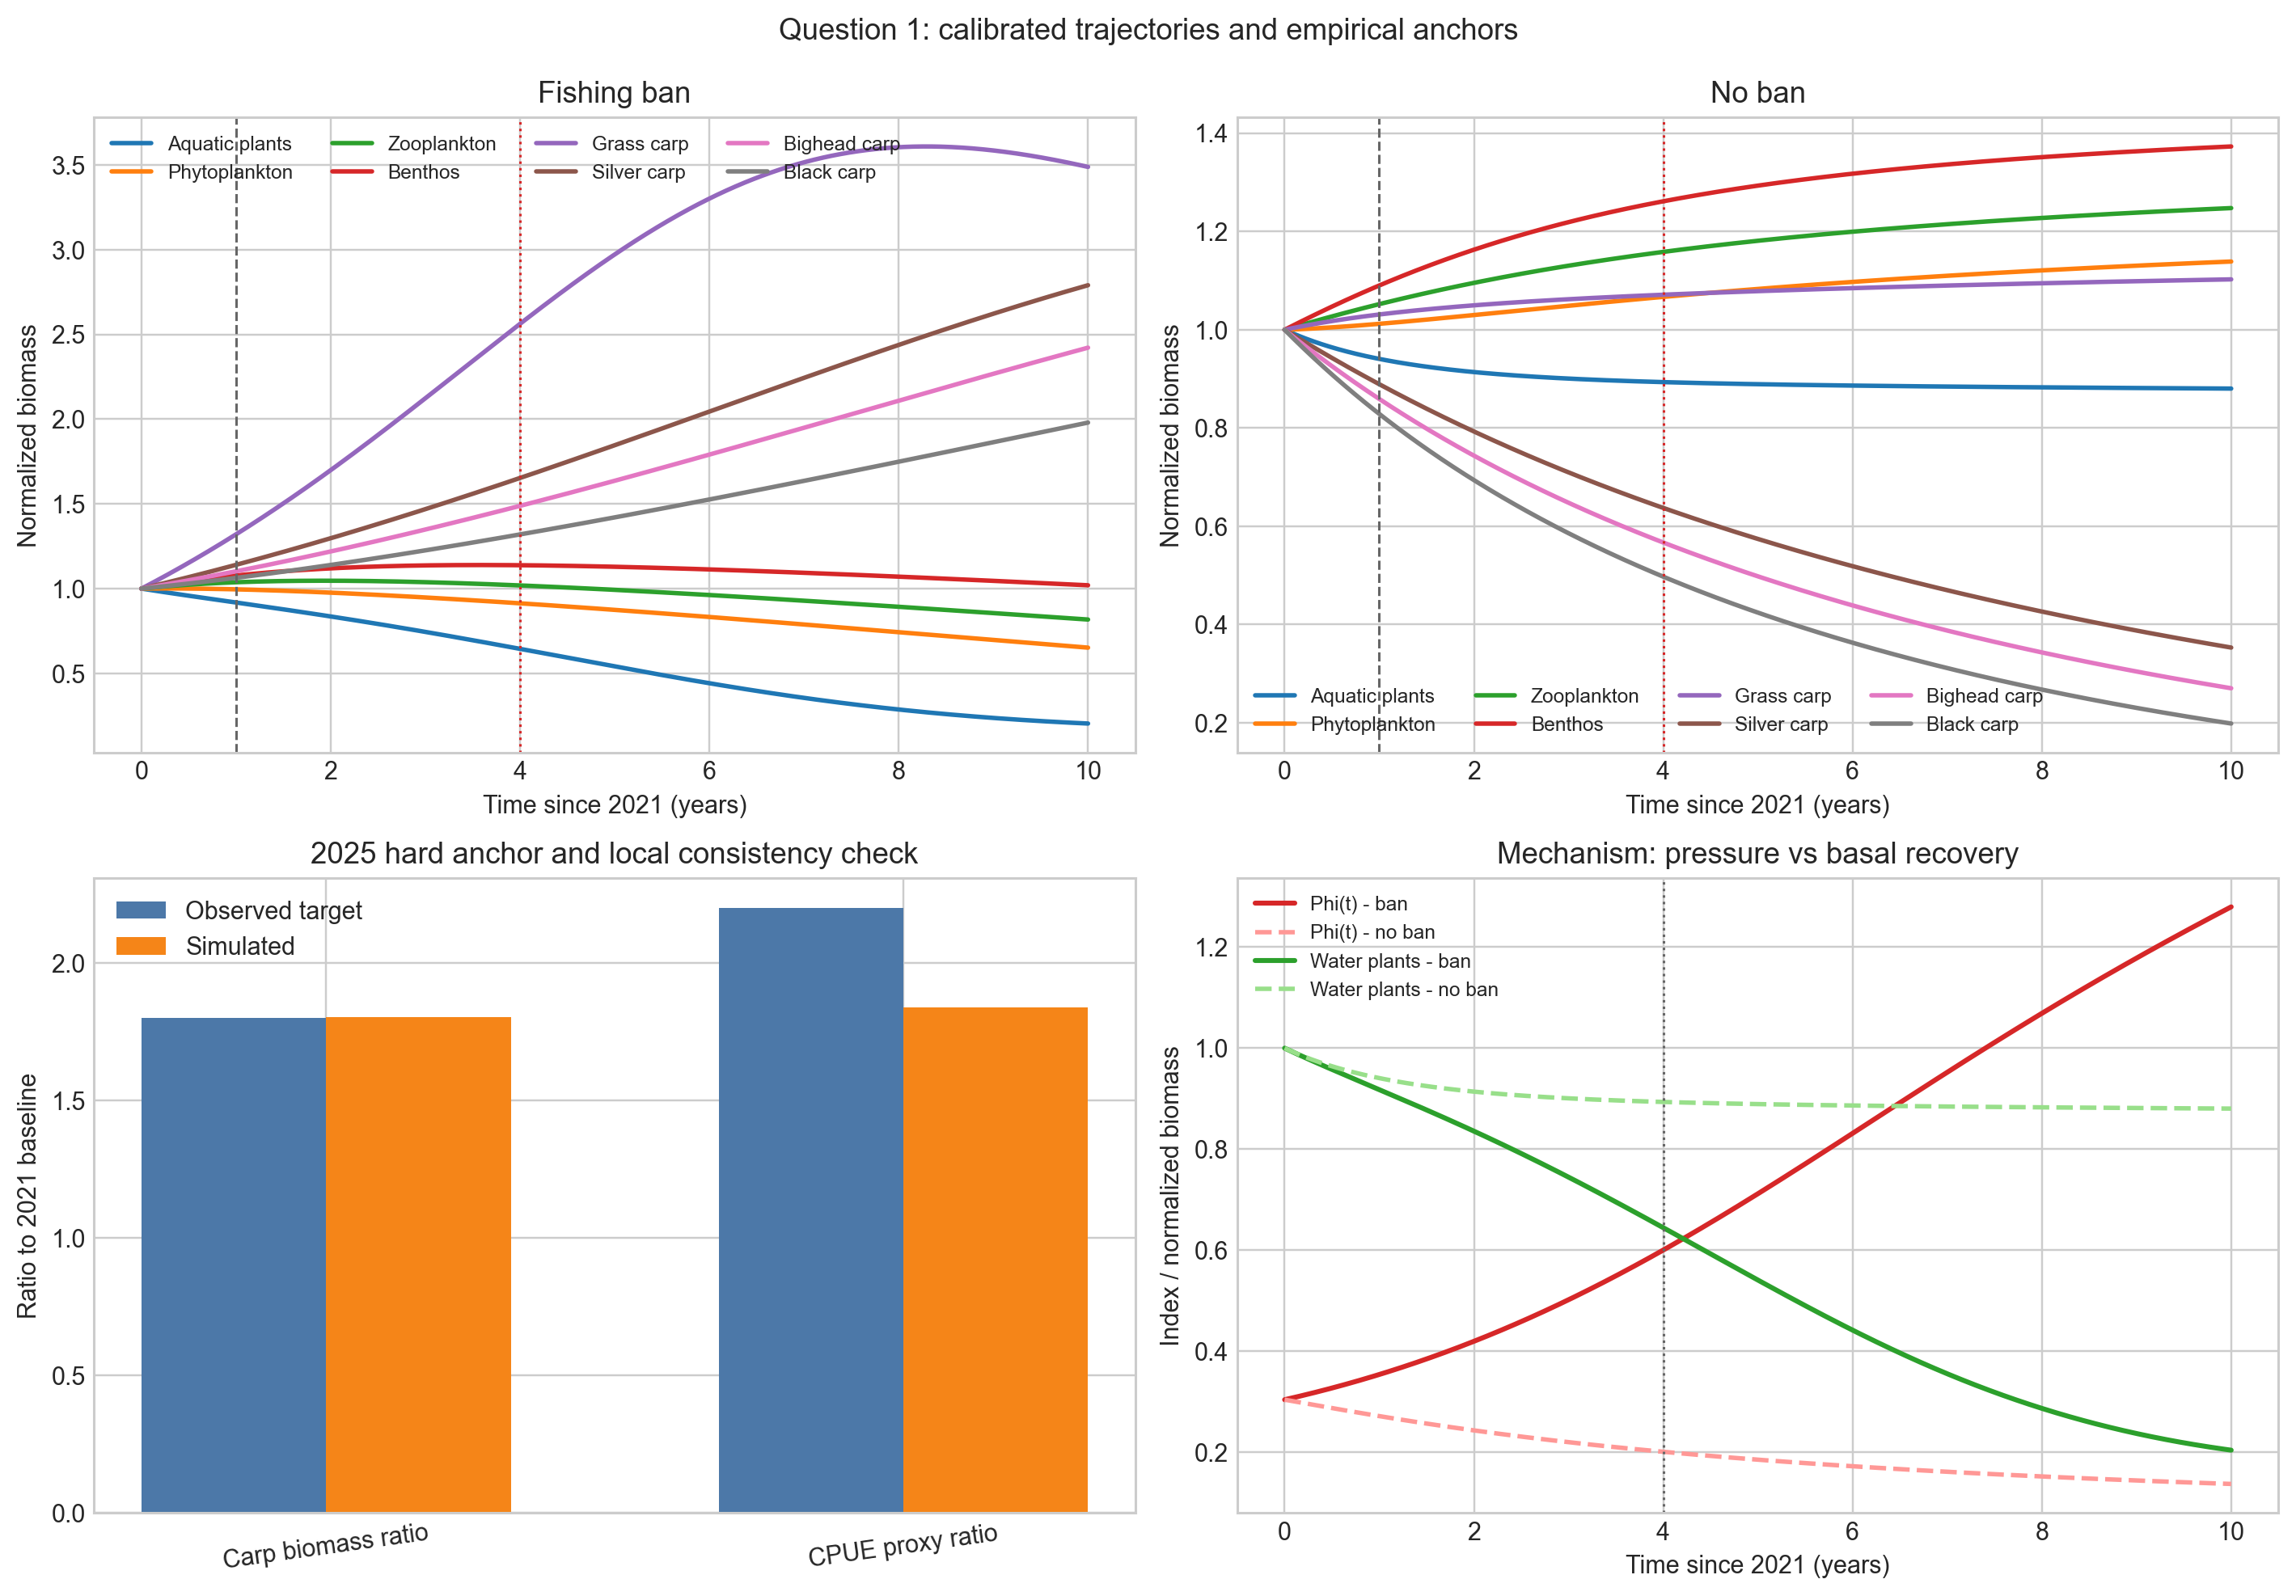
\includegraphics[width=0.92\textwidth]{fig01_q1_foodweb.png}
\caption{问题一：标定后的禁渔与对照情景及观测约束}
\label{fig:q1}
\end{figure}

\section{问题二的模型建立与求解}
\subsection{模型建立}
我们在问题二中以问题一得到的上游资源-鱼群动态轨迹作为输入，在统一初始条件下构建珍稀物种种群响应子模型，并通过对照情景分离食源供给、江湖连通性与人工放流的独立效应。其中变量$M$不再以四大家鱼作为对应对象，而是代表长江江豚与长江鲟共享的中层猎物库，涵盖四大家鱼以外的中小型鱼类、幼鱼及鱼虾混合饵料；$D$和$A$分别表示长江江豚与长江鲟种群，$V$表示外来入侵竞争物种。

问题一的动力系统旨在刻画禁渔对基础资源层和经济鱼类的恢复过程，而问题二聚焦于珍稀保护物种可利用的公共食源库，二者研究对象与生态位并不完全对应。因此上游生态信息通过综合生态状态指数$E(t)$驱动中层猎物承载力$K_M$，而非将四大家鱼的种群状态直接赋值为$M$。研究情景与模型设定的对应关系如表 \ref{tab:q2map} 所示。
\begin{table}[htbp]
\centering
\caption{问题二的观测事实与模型映射}
\label{tab:q2map}
\begin{tabularx}{0.95\textwidth}{>{\raggedright\arraybackslash}p{2.4cm} >{\raggedright\arraybackslash}p{4.2cm} >{\raggedright\arraybackslash}p{3.6cm} X}
\toprule
事实来源 & 观测口径 & 对应模型量 & 角色 \\
\midrule
附件 1 & 洄游路径、大坝阻隔、鱼道连通性 & $\delta_B$ & 事实约束 \\
附件 2 & 食性分工 & $a_D,a_A,a_V$ & 经验参数设定 \\
附件 2 & 放流补偿 & $R_A$ & 情景量 \\
附件 3（2022 公报） & 江豚 1249 头、长江鲟 438 尾 & $D(0),A(0)$ & 初值约束 \\
问题一输出 & 归一化生态指数 $E(t)$ & $E(t)$ & 上游输入量 \\
\bottomrule
\end{tabularx}
\end{table}
其中 $\delta_B,D(0),A(0)$ 直接对应题目事实；$a_D,a_A,a_V$ 为经验参数，$R_A$ 为情景控制量（取值 0.012，对应附件 2 中长江鲟年均放流规模与 2022 公报存量的比值），$E(t)$ 作为问题一输出的上游输入量使用。高阻隔情景提高 $\delta_B$，无放流情景取 $R_A=0$，污染情景提高 $u$，其余参数保持不变。

对任一状态量 $X$ 记 $\widetilde X(t)=X(t)/X(0)$。由问题一得到底层资源和四大家鱼轨迹后，我们构造综合生态状态指数
\begin{equation}
E(t)=0.62E_{\text{basal}}(t)+0.38E_{\text{carp}}(t),
\end{equation}
\begin{equation}
E_{\text{basal}}(t)=0.30\widetilde W(t)+0.25\widetilde{Ph}(t)+0.25\widetilde Z(t)+0.20\widetilde N(t),
\end{equation}
\begin{equation}
E_{\text{carp}}(t)=0.28\widetilde G(t)+0.24\widetilde L(t)+0.24\widetilde Y(t)+0.24\widetilde Q(t).
\end{equation}
其中 $E_{\text{basal}}$ 保留资源端压力信号，$E_{\text{carp}}$ 保留鱼群恢复信号。权重 0.62 和 0.38 用于同时保留这两部分信息：在问题一的标定轨迹上，2025 年 $E_{\text{basal}}=0.904$、$E_{\text{carp}}=1.788$，若完全依赖鱼群层，$E(t)$ 会趋近于单纯的鱼群恢复指标，从而削弱资源端信息。将 $E_{\text{basal}}$ 权重在 $[0.50,0.75]$ 范围内扫描后，基线情景下江豚和长江鲟末值的最大变动分别仅为 1.21\% 和 0.18\%，四组情景中的物种排序和作用方向保持不变。为使中层猎物承载力同时响应食源恢复和污染压力，按脚本实现取
\begin{equation}
K_M(E,u)=\max\left\{0.18,\;k_M\bigl(0.62+0.76E(t)\bigr)\max\bigl(0.30,1-0.60u\bigr)\right\},
\end{equation}
其中基准取 $k_M=1$。$K_M(E,u)$ 在此作为由上游轨迹诱导的一维食源强迫项，汇集问题一中的恢复与退化信号。建立珍稀物种与入侵物种模型\cite{holling1959}：
\begin{equation}
\frac{\mathrm{d}M}{\mathrm{d}t}
=r_M M\left(1-\frac{M}{K_M(E,u)}\right)
-a_D\frac{MD}{1+h_MM}
-a_A\frac{MA}{1+h_MM}
-a_V\frac{MV}{1+h_MM}
-\lambda_u uM,
\end{equation}
\begin{equation}
\frac{\mathrm{d}D}{\mathrm{d}t}
=e_D a_D\frac{MD}{1+h_MM}-(m_D+\delta_B+\mu_Du)D,
\end{equation}
\begin{equation}
\frac{\mathrm{d}A}{\mathrm{d}t}
=R_A+e_A a_A\frac{MA}{1+h_MM}-(m_A+\gamma_B\,\delta_B+\mu_Au)A,
\end{equation}
\begin{equation}
\frac{\mathrm{d}V}{\mathrm{d}t}
=e_V a_V\frac{MV}{1+h_MM}-(m_V+\mu_Vu)V.
\end{equation}
式中 $\delta_B$ 表示通道阻隔和栖息地碎片化的综合损失，$R_A$ 表示人工放流强度，$\gamma_B$ 表示长江鲟阻隔敏感性放大因子，基准取 $\gamma_B=1.3$。考虑到长江鲟属洄游型鱼类，其繁殖和生长对通道连通性的依赖显著高于定居型的江豚，模型中对阻隔项作适度放大；附件 1 给出的信息显示，长江鲟洄游距离约为江豚日常活动范围的 1.3 倍，这一数值也为 $\gamma_B$ 的基准取值提供了参照。将该乘数在 $[1.1,1.5]$ 范围内扫描后，基线情景下长江鲟末值的最大变动约为 2.1\%，四组情景中长江鲟的排序保持不变，说明结论对该乘数的具体取值不敏感。题目事实与模型口径的对应关系已在表 \ref{tab:q2map} 中统一给出。

\subsection{情景结果与机制讨论}
在2022公报归一化口径下，基线情景的江豚和长江鲟末值为1.133和1.140。若只增强通道阻隔、暂不叠加额外污染，二者降至0.901和0.856。把长江鲟放流项置为$R_A=0$后，长江鲟降至0.519，而江豚仅变为1.145；污染情景下，两者又降至0.610和0.704。这里改变的是通道损失参数和放流控制量；放流项位于长江鲟方程，通道损失同时进入两类物种方程。通道约束同时压低两类物种，放流变化主要落在长江鲟上。表中报告江豚和长江鲟终态，$M$与$V$留作后文解释过程差异。
\begin{table}[htbp]
\centering
\caption{问题二的结果口径、相对变化与对照说明}
\label{tab:q2_result}
\begin{tabularx}{0.95\textwidth}{>{\raggedright\arraybackslash}p{2.2cm} >{\raggedright\arraybackslash}p{3.6cm} >{\raggedright\arraybackslash}p{2.8cm} >{\raggedright\arraybackslash}p{1.7cm} X}
\toprule
项目 & 数值/情景输出 & 相对基线变化 & 是否外部验证 & 解释用途 \\
\midrule
2022 公报基准 & 江豚 1249 头、长江鲟 438 尾 & -- & 是 & 作为问题二的初值与口径基准 \\
基线情景末值 & 江豚 1.133，长江鲟 1.140 & -- & 否 & 作为禁渔与食源修复下的基线投影 \\
$R_A=0$ 对照 & 江豚 1.145，长江鲟 0.519 & 江豚 +1.0\%，长江鲟 -54.5\% & 否 & 拆分自然恢复与人工放流补偿效应 \\
高阻隔对照 & 江豚 0.901，长江鲟 0.856 & 江豚 -20.5\%，长江鲟 -24.9\% & 否 & 仅提高通道阻隔，分离生境约束效应 \\
污染情景末值 & 江豚 0.610，长江鲟 0.704 & 江豚 -46.2\%，长江鲟 -38.2\% & 否 & 比较污染叠加阻隔对基线收益的侵蚀 \\
\bottomrule
\end{tabularx}
\end{table}
这些对照对应的机制各有差异。无放流时，长江鲟大幅下降而江豚变化很小，说明人工补偿主要作用于鲟类而不是江豚；高阻隔与污染情景同时压低两类物种，说明连通性和环境质量属于共性约束。作为定性验证，模型在$t=3$（对应2024年）时已有$A(3)/A(0)>1$，与题目所述“2024 年长江鲟自然繁殖群体重新出现产卵场”这一事实方向一致。

\paragraph{参数敏感性分析}
为检验情景结论对经验参数的依赖程度，对 6 个关键参数分别施加 $\pm 20\%$ 扰动，记录终态江豚 $D$ 和长江鲟 $A$ 相对基线的变化率（表 \ref{tab:q2_sens}）。

\begin{table}[htbp]
\centering
\caption{问题二参数敏感性分析（$\pm 20\%$ 扰动）}
\label{tab:q2_sens}
\begin{tabular}{lcccc}
\toprule
参数 & $\Delta D_{+20\%}$ & $\Delta D_{-20\%}$ & $\Delta A_{+20\%}$ & $\Delta A_{-20\%}$ \\
\midrule
$\delta_B$（通道阻隔） & $-1.9\%$ & $+2.0\%$ & $-2.5\%$ & $+2.6\%$ \\
$R_A$（放流强度） & $-0.2\%$ & $+0.2\%$ & $+10.9\%$ & $-10.9\%$ \\
$e_D$（江豚转化率） & $+8.3\%$ & $-9.4\%$ & $-0.8\%$ & $+0.9\%$ \\
$e_A$（长江鲟转化率） & $-0.0\%$ & $+0.0\%$ & $+1.8\%$ & $-1.8\%$ \\
$a_D$（江豚摄食率） & $-8.5\%$ & $+5.2\%$ & $-2.7\%$ & $+3.6\%$ \\
$a_A$（长江鲟摄食率） & $-0.8\%$ & $+0.8\%$ & $+1.7\%$ & $-1.7\%$ \\
\bottomrule
\end{tabular}
\end{table}

敏感性结果显示，江豚终态对 $e_D$ 和 $a_D$ 最敏感（$|\Delta D|>5\%$），说明江豚恢复对食物获取效率变化最为敏感。长江鲟那边最显眼的是放流强度 $R_A$（$|\Delta A|\approx 11\%$），人工放流仍是恢复中的关键补偿项。通道阻隔 $\delta_B$ 对两物种都有负面影响，只是放到当前参数区间里看，扰动幅度还没有前两者那么大（$<3\%$）。

\begin{figure}[htbp]
\centering
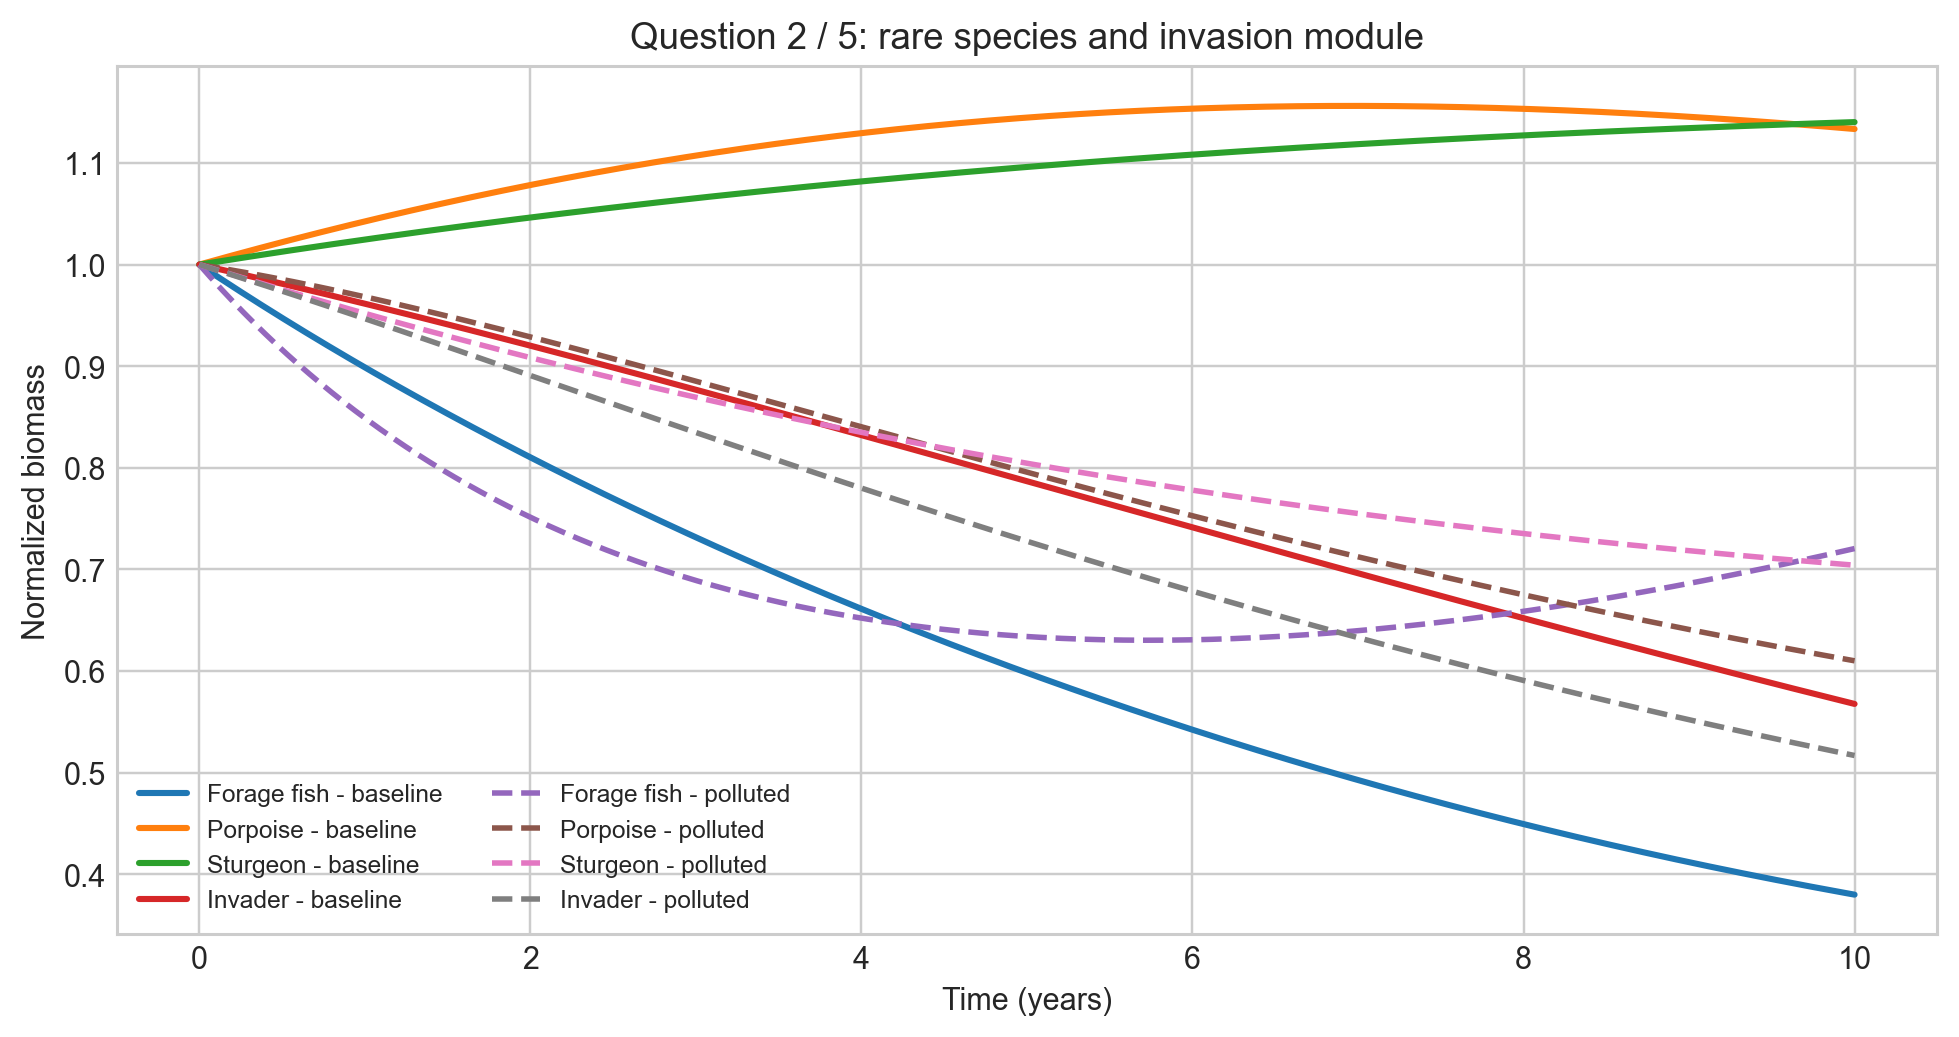
\includegraphics[width=0.88\textwidth]{fig02_q2_rare_species.png}
\caption{问题二和问题五共用的稀有种与入侵模块结果}
\label{fig:q2}
\end{figure}

\section{问题三的模型建立与求解}
\subsection{模型建立}
在这一问里，我们把长期动力学部分压缩为 Hastings-Powell 三级食物链这一最小闭环，在同一参数轴上比较“资源--消费者--捕食者”反馈下的轨道类型\cite{hp1991}：
\begin{equation}
\frac{\mathrm{d}X_1}{\mathrm{d}t}
=rX_1\left(1-\frac{X_1}{K}\right)-\frac{a_1X_1X_2}{b_1+X_1},
\end{equation}
\begin{equation}
\frac{\mathrm{d}X_2}{\mathrm{d}t}
=\frac{a_1X_1X_2}{b_1+X_1}-\frac{a_2X_2X_3}{b_2+X_2}-d_1X_2,
\end{equation}
\begin{equation}
\frac{\mathrm{d}X_3}{\mathrm{d}t}
=\frac{a_2X_2X_3}{b_2+X_2}-d_2X_3.
\end{equation}
其中 $K$ 代表基础食物链有效承载力，可理解为营养输入、水质改善或污染冲击后的综合结果。物种映射上，$X_1$ 对应底层资源层（问题一中 $R_j$ 的聚合），$X_2$ 对应中层消费者（四大家鱼功能群），$X_3$ 对应顶层捕食者（江豚等）。我们在这里仅保留营养级对应，用于说明三级食物链的生态位含义，不直接继承问题一的参数数值。

模型参数取值如表 \ref{tab:q3_hp_params} 所示，其中 $a_1,b_1,d_1$ 和 $a_2,b_2,d_2$ 分别控制中层和顶层的摄食与损失，$r$ 固定为 1，$K$ 作为扫描控制参数。
\begin{table}[htbp]
\centering
\caption{问题三的 Hastings-Powell 模型参数取值}
\label{tab:q3_hp_params}
\begin{tabularx}{0.85\textwidth}{>{\raggedright\arraybackslash}p{1.5cm} >{\centering\arraybackslash}p{1.5cm} X}
\toprule
参数 & 取值 & 说明 \\
\midrule
$r$ & 1.0 & 底层资源内禀增长率，固定为归一化基准 \\
$a_1$ & 5.0 & 中层对底层的摄食率，取自 Hastings \& Powell (1991) 默认值\cite{hp1991} \\
$b_1$ & 1.0 & 中层摄食半饱和常数 \\
$a_2$ & 0.1 & 顶层对中层的摄食率 \\
$b_2$ & 2.0 & 顶层摄食半饱和常数 \\
$d_1$ & 0.4 & 中层自然死亡率 \\
$d_2$ & 0.01 & 顶层自然死亡率 \\
$K$ & 扫描 & 承载力控制参数，扫描范围 $[1.4,4.8]$ \\
\bottomrule
\end{tabularx}
\end{table}

\subsection{求解与结果}
参数 $K$ 表示三级食物链的综合承载条件。固定当前参数组并取代表点后，$K\approx 1.8$ 附近对应规则有界振荡，$K\approx 2.7$ 附近对应明显周期振荡；更高 $K$ 下轨道会呈现更不规则的波动，但严格的混沌识别留到问题四通过最大李雅普诺夫指数完成。后期统计量统一在积分后期时间窗 $t\in[90,180]$ 上提取，包括 $X_1$ 的峰谷差 $\Delta X_1$、平均峰间隔 $\bar T$ 和峰间隔变异系数 $\mathrm{CV}_T$，如表 \ref{tab:q3traj} 所示。

统计量限定在积分后期时间窗内计算，以滤除初值诱发的瞬态影响。由此得到的 $\sigma(X_1)$、$\Delta X_1$ 与 $\mathrm{CV}_T$ 才能用于不同 $K$ 之间的轨道比较。

\begin{table}[htbp]
\centering
\caption{问题三代表轨道的积分后期描述量}
\label{tab:q3traj}
\small
\begin{tabularx}{0.95\textwidth}{>{\raggedright\arraybackslash}p{2.9cm} >{\centering\arraybackslash}p{1.2cm} >{\centering\arraybackslash}p{1.4cm} >{\centering\arraybackslash}p{1.4cm} >{\centering\arraybackslash}p{1.3cm} >{\centering\arraybackslash}p{1.5cm} >{\centering\arraybackslash}p{1.4cm}}
\toprule
类型 & $K$ & $\sigma(X_1)$ & $\Delta X_1$ & $N_{\text{peak}}$ & $\bar T$ & $\mathrm{CV}_T$ \\
\midrule
规则有界振荡 & 1.795 & 0.261 & 0.991 & 4 & 20.720 & 0.004 \\
明显周期振荡 & 2.665 & 0.502 & 2.092 & 3 & 34.178 & 0.014 \\
复杂非线性波动 & 4.800 & 0.885 & 4.093 & 13 & 4.298 & 2.746 \\
\bottomrule
\end{tabularx}
\normalsize
\end{table}

随着 $K$ 增大，$X_1$ 的标准差由 0.261 升至 0.885，峰谷差由 0.991 扩大到 4.093，而峰间隔变异系数由 0.004 升至 2.746，说明系统从规则振荡逐步走向更复杂的长期行为。第三行仅作为复杂非线性波动样本展示，不在问题三中单独给出混沌判断；相关判据仍由问题四的李雅普诺夫扫描提供。图 \ref{fig:q3} 给出三类代表轨道。

\begin{figure}[htbp]
\centering
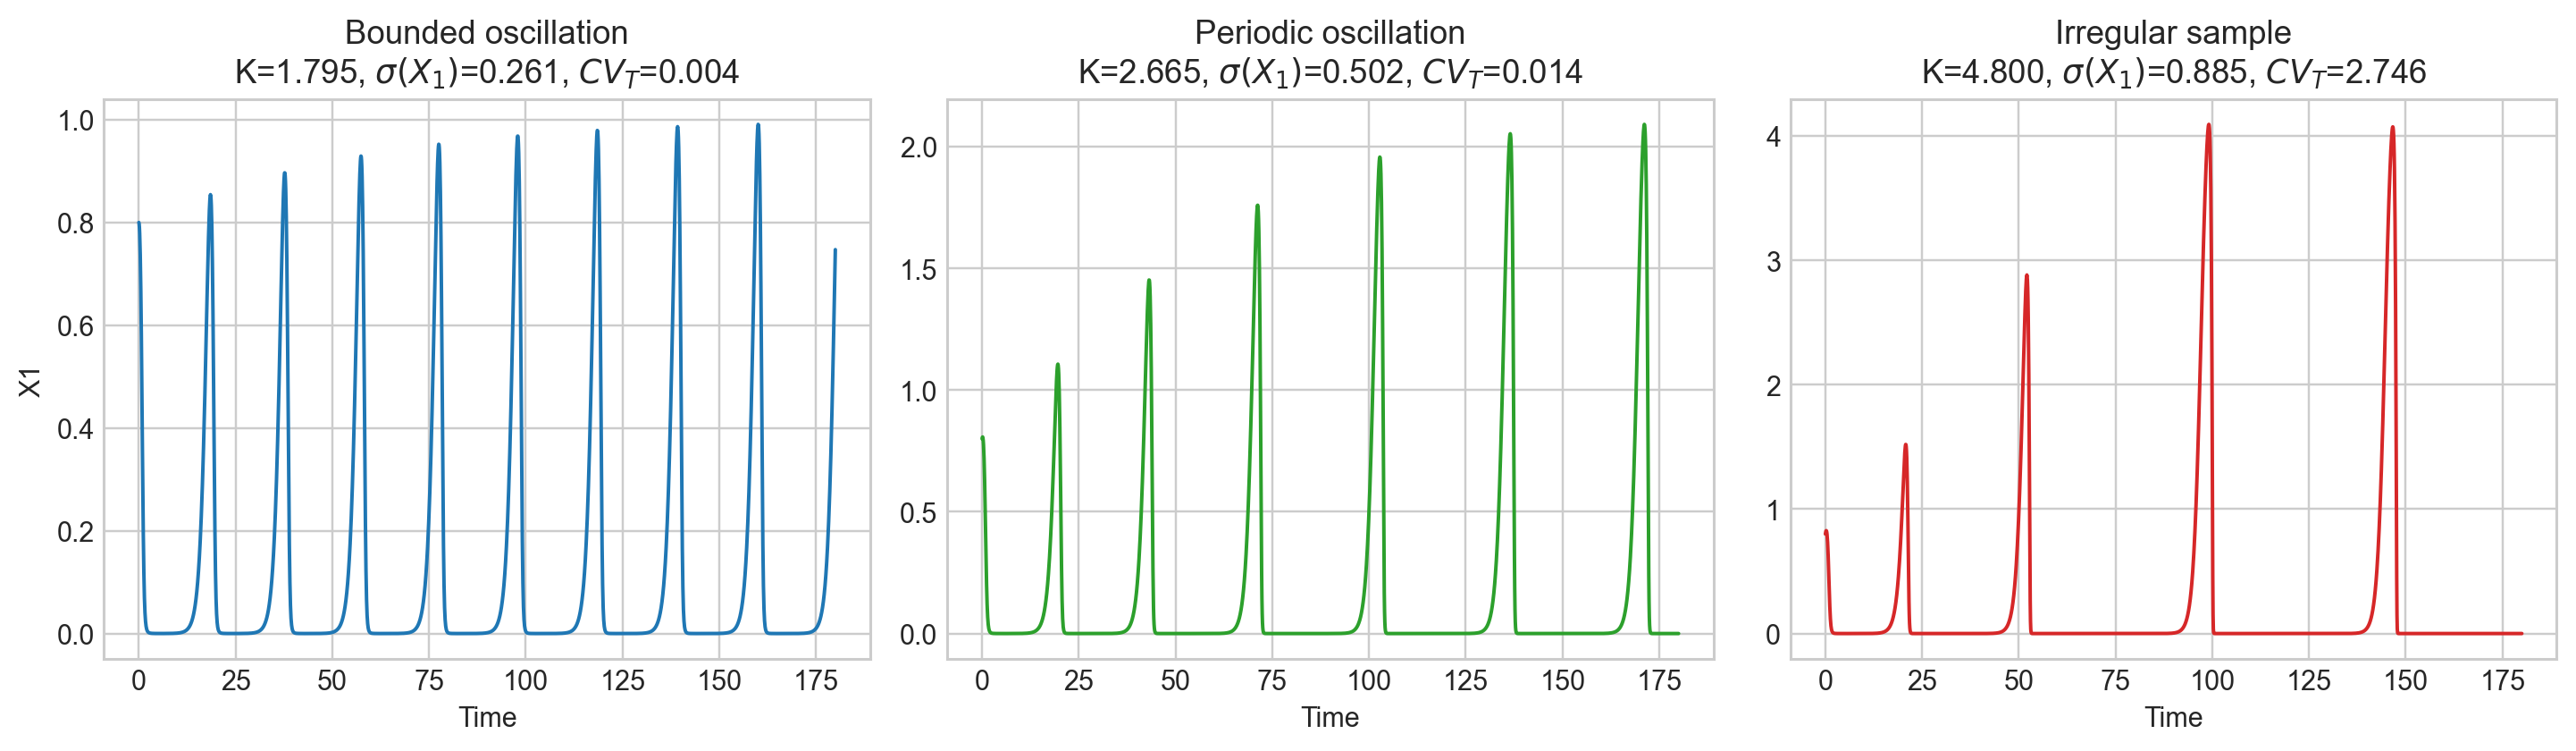
\includegraphics[width=0.96\textwidth]{fig03_q3_hastings_powell.png}
\caption{问题三代表轨道示意}
\label{fig:q3}
\end{figure}

\section{问题四的模型建立与求解}
\subsection{模型建立}
我们在问题四中沿用问题三的方程组和参数集，仅将判别工具替换为 Benettin 型有限时间最大李雅普诺夫指数 $\lambda_{\max}$。数值实现中，先由 Hastings-Powell 方程写出解析 Jacobian，再将状态方程与切向方程用四阶 Runge--Kutta 同步积分，并在每个时间步对切向向量进行一次归一化；“瞬态截断 40”指前 40 个时间单位的轨道不进入指数累计。基准设置取初值 $(0.8,0.2,0.2)$、步长 $dt=0.01$ 和总积分时长 90；同时将总积分时长扩展到 150 和 200，并在 $K=3.20$ 与 $K=3.22$ 附近做局部步长和初值复核，用以检验正指数起点对数值设置的敏感性。

\subsection{求解与结果}
基准时间窗下，$\lambda_{\max}$先在1.4--4.8粗网格上扫描，再在3.0--3.4加密。首个连续正区间位于$K=3.2186$附近，3.22--3.40保持为正。表\ref{tab:q4robust}表明，在总积分时长固定为90的前提下，$K=3.20$与$K=3.22$之间的符号跨越在相邻步长和微扰初值下仍可保留。

\begin{table}[htbp]
\centering
\caption{问题四短时间窗局部复核}
\label{tab:q4robust}
\small
\begin{tabularx}{0.95\textwidth}{>{\raggedright\arraybackslash}p{4.1cm} >{\centering\arraybackslash}p{1.9cm} >{\centering\arraybackslash}p{1.9cm} >{\centering\arraybackslash}p{1.9cm} X}
\toprule
设置 & $\lambda_{\max}(3.20)$ & $\lambda_{\max}(3.22)$ & 判别 & 说明 \\
\midrule
基准步长 $dt=0.010$ & $-0.00135$ & $0.00117$ & 符号跨越 & 3.22 附近进入正指数区间 \\
较小步长 $dt=0.008$ & $-0.00134$ & $0.00117$ & 符号跨越 & 结果与基准设置一致 \\
较大步长 $dt=0.012$ & $-0.00129$ & $0.00123$ & 符号跨越 & 结果与基准设置一致 \\
微扰初值 $(0.8005,0.1995,0.2)$ & $-0.00087$ & $0.00165$ & 符号跨越 & 微扰后仍保留同样的符号关系 \\
\bottomrule
\end{tabularx}
\normalsize
\end{table}

积分时长改变后，短窗口给出的起点发生移动。时长150时，3.0--3.4加密区间全部为正；时长200时，连续正区间从3.11开始，$\lambda_{\max}(3.20)=0.00579$、$\lambda_{\max}(3.22)=0.00701$也都为正。由5组初值、5个步长和3个积分时长组成的75组测试中，仅5组（6.7\%）保留$\lambda_{\max}(3.20)<0<\lambda_{\max}(3.22)$。该局部跨越在扩展设置下不具备统计稳健性。

基准短时间窗下，$K=3.2186$附近出现局部跨越；积分时长和数值设置放宽后，这个跨越难以保持，不能说明起点固定，因此$K=3.2186$不能作为唯一临界点。本文据此只保留“承载力提高会增强系统复杂性”的方向性判断；若要定位分岔值，仍须采用更长积分时长（$\ge 500$）并配合分岔图。图\ref{fig:q4}给出不同积分时长下的有限时间指数。

\begin{figure}[htbp]
\centering
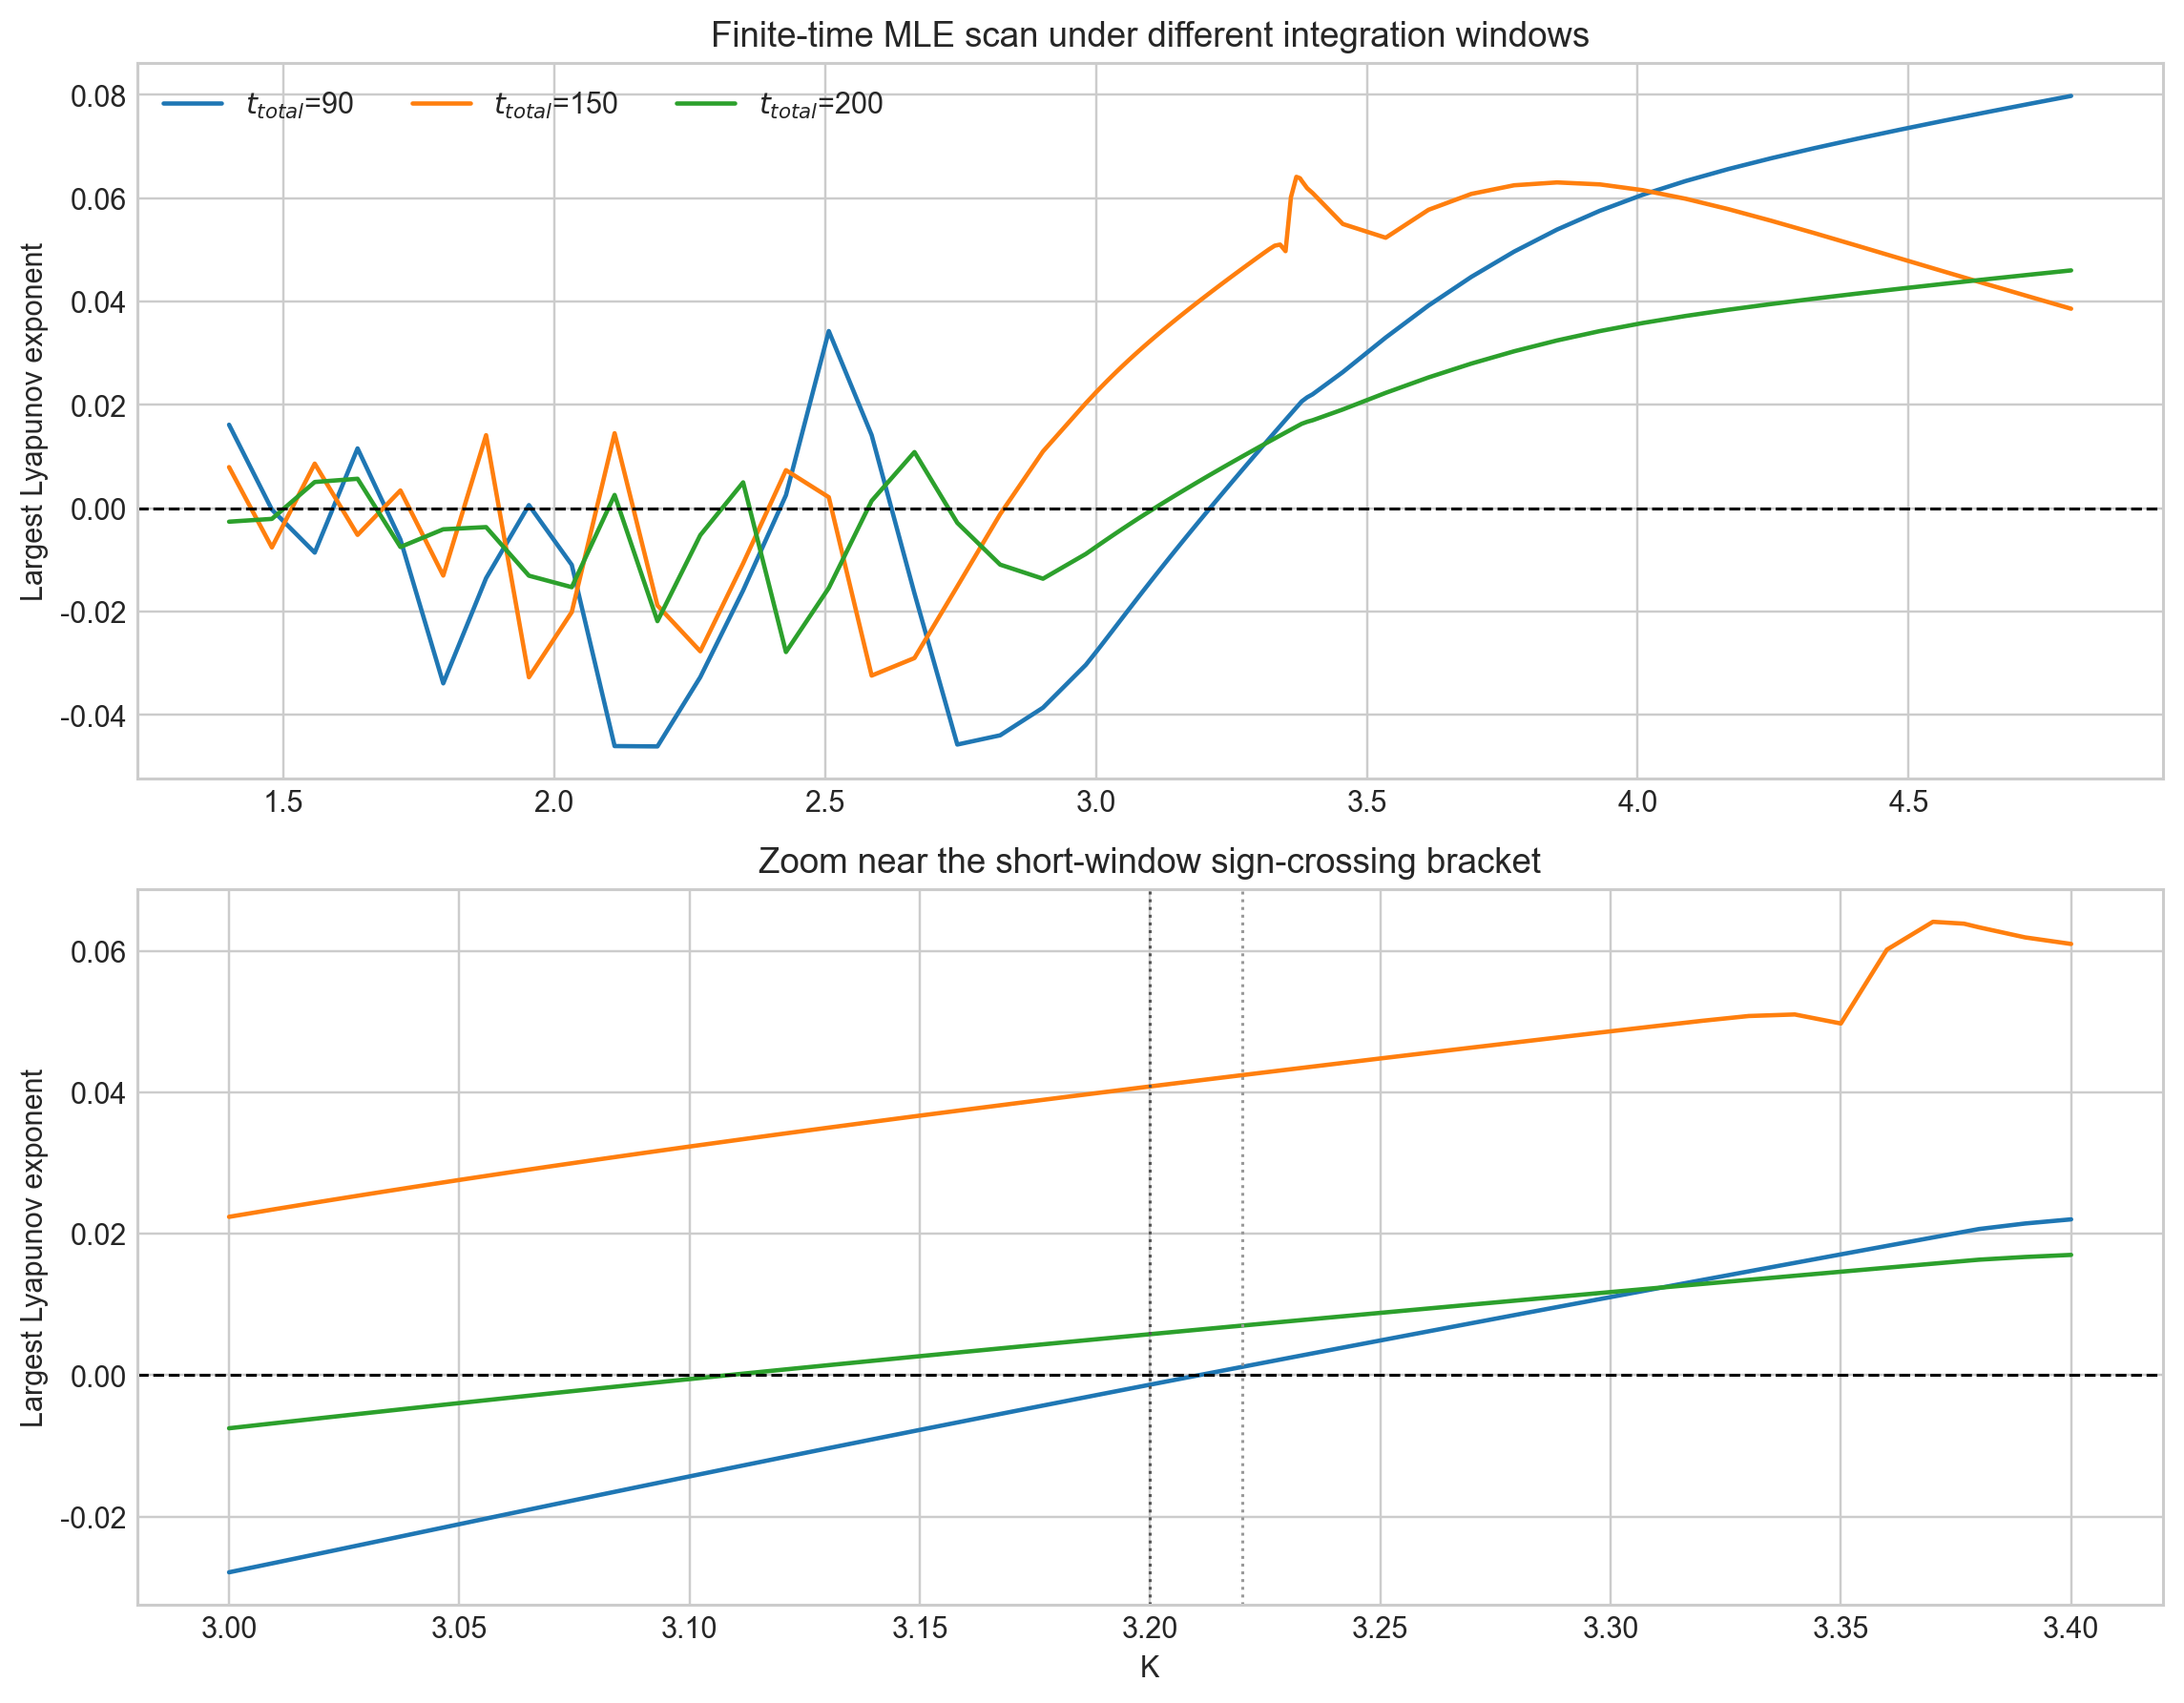
\includegraphics[width=0.92\textwidth]{fig04_q4_lyapunov_scan.png}
\caption{问题四不同积分时长下的有限时间李雅普诺夫指数扫描}
\label{fig:q4}
\end{figure}

\section{问题五的模型建立与求解}
\subsection{模型建立}
我们在问题五中沿用问题二的状态方程，并在污染强度、入侵初值和竞争强度上做情景扩展。由于问题一的基线轨迹对应 $u=0$，污染情景下的上游输入需要再次由问题一积分得到，以便使资源退化、鱼群变化与污染设定保持一致。具体而言，先以 $u>0$ 重新计算 $E_{\text{basal}}$ 和 $E_{\text{carp}}$，再将其输入问题二模块。

考虑到污染和入侵会诱发幅度较大的波动，我们统一比较积分后期最后 200 个离散采样点上的平均指标，以减弱瞬时相位的影响。设第 $i$ 个情景在该尾窗上的四个平均指标分别为 $\bar M_i,\bar D_i,\bar A_i,\bar V_i$，其中食源、江豚和长江鲟为效益型指标，入侵压力为成本型指标。先对三种情景构造正向化指标矩阵，再分别计算熵权和 CRITIC 权重，并取两者平均作为组合权重。记组合权重为 $w=(w_1,w_2,w_3,w_4)$，则综合得分定义为
\begin{equation}
\mathcal{H}_i=\sum_{j=1}^{4}w_j z_{ij},\qquad \sum_{j=1}^{4}w_j=1,\quad w_j\ge 0.
\end{equation}
在当前数据下，组合权重为 $(0.232,0.289,0.298,0.181)$，分别对应食源、江豚、长江鲟和入侵压力。该指标用于比较三种情景的相对状态，不对应外部生态健康的绝对量值。

\subsection{求解与结果}
表\ref{tab:q5result}列出“仅禁渔”、“禁渔+污染”和“禁渔+污染+入侵”的尾窗均值。三类指标并不同步：综合得分依次为0.662、0.423和0.155；与仅禁渔相比，污染情景的食源由0.407升至0.692，江豚和长江鲟却降至0.636和0.716；污染上再加入侵后，入侵压力达到0.641，综合得分继续下降。
\begin{table}[htbp]
\centering
\caption{问题五的积分后期平均指标与综合得分}
\label{tab:q5result}
\begin{tabularx}{0.95\textwidth}{>{\raggedright\arraybackslash}p{3.0cm} >{\centering\arraybackslash}p{1.6cm} >{\centering\arraybackslash}p{1.6cm} >{\centering\arraybackslash}p{1.6cm} >{\centering\arraybackslash}p{1.6cm} >{\centering\arraybackslash}p{1.6cm}}
\toprule
情景 & 食源 & 江豚 & 长江鲟 & 入侵压力 & $\mathcal{H}$ \\
\midrule
仅禁渔 & 0.407 & 1.143 & 1.135 & 0.602 & 0.662 \\
禁渔+污染 & 0.692 & 0.636 & 0.716 & 0.546 & 0.423 \\
禁渔+污染+入侵 & 0.598 & 0.624 & 0.711 & 0.641 & 0.155 \\
\bottomrule
\end{tabularx}
\end{table}
\begin{table}[htbp]
\centering
\caption{问题五的赋权结果与排序稳健性}
\label{tab:q5_weight}
\small
\setlength{\tabcolsep}{2pt}
\begin{tabularx}{0.95\textwidth}{>{\raggedright\arraybackslash}p{2.2cm} >{\raggedright\arraybackslash}p{4.3cm} >{\raggedright\arraybackslash}p{3.5cm} X}
\toprule
方案 & 权重 $(M,D,A,V)$ & 排序结果 & 说明 \\
\midrule
熵权 & $(0.144,0.337,0.351,0.168)$ & 仅禁渔 \textgreater 禁渔+污染 \textgreater 禁渔+污染+入侵 & 根据指标离散程度确定权重 \\
CRITIC & $(0.319,0.242,0.244,0.194)$ & 仅禁渔 \textgreater 禁渔+污染 \textgreater 禁渔+污染+入侵 & 同时考虑对比强度与相关性 \\
组合权重 & $(0.232,0.289,0.298,0.181)$ & 仅禁渔 \textgreater 禁渔+污染 \textgreater 禁渔+污染+入侵 & 取熵权与 CRITIC 权重的平均值 \\
等权对照 & $(0.250,0.250,0.250,0.250)$ & 仅禁渔 \textgreater 禁渔+污染 \textgreater 禁渔+污染+入侵 & 用于检查排序是否依赖某一套客观权重 \\
局部扰动 & -- & 仅禁渔 \textgreater 禁渔+污染 \textgreater 禁渔+污染+入侵 & 围绕组合权重做 2000 次 $[0.85,1.15]$ 重归一扰动，完整排序稳定率为 100\% \\
\bottomrule
\end{tabularx}
\normalsize
\end{table}
污染情景中食源指标抬升而江豚、长江鲟同步下降，反映的是当前参数组下的捕食释放机制。方程中，$u$一方面下压$K_M$，另一方面以较大幅度抬升两类珍稀物种的死亡项；后者造成的捕食减少在尾窗内超过了承载损失，于是$M$均值短时回升。这个回升只对应过程量的再分配，不意味着污染改善了系统健康。

熵权、CRITIC、等权和组合赋权得到同一排序，组合权重经2000 次$[0.85,1.15]$重归一扰动后，完整排序稳定率与“入侵情景最差”稳定率均为100\%。不同赋权下比较关系都没有改变，因此污染削弱禁渔收益、入侵继续增加压力的次序判断并不依赖某一套特定赋权。

\begin{figure}[htbp]
\centering
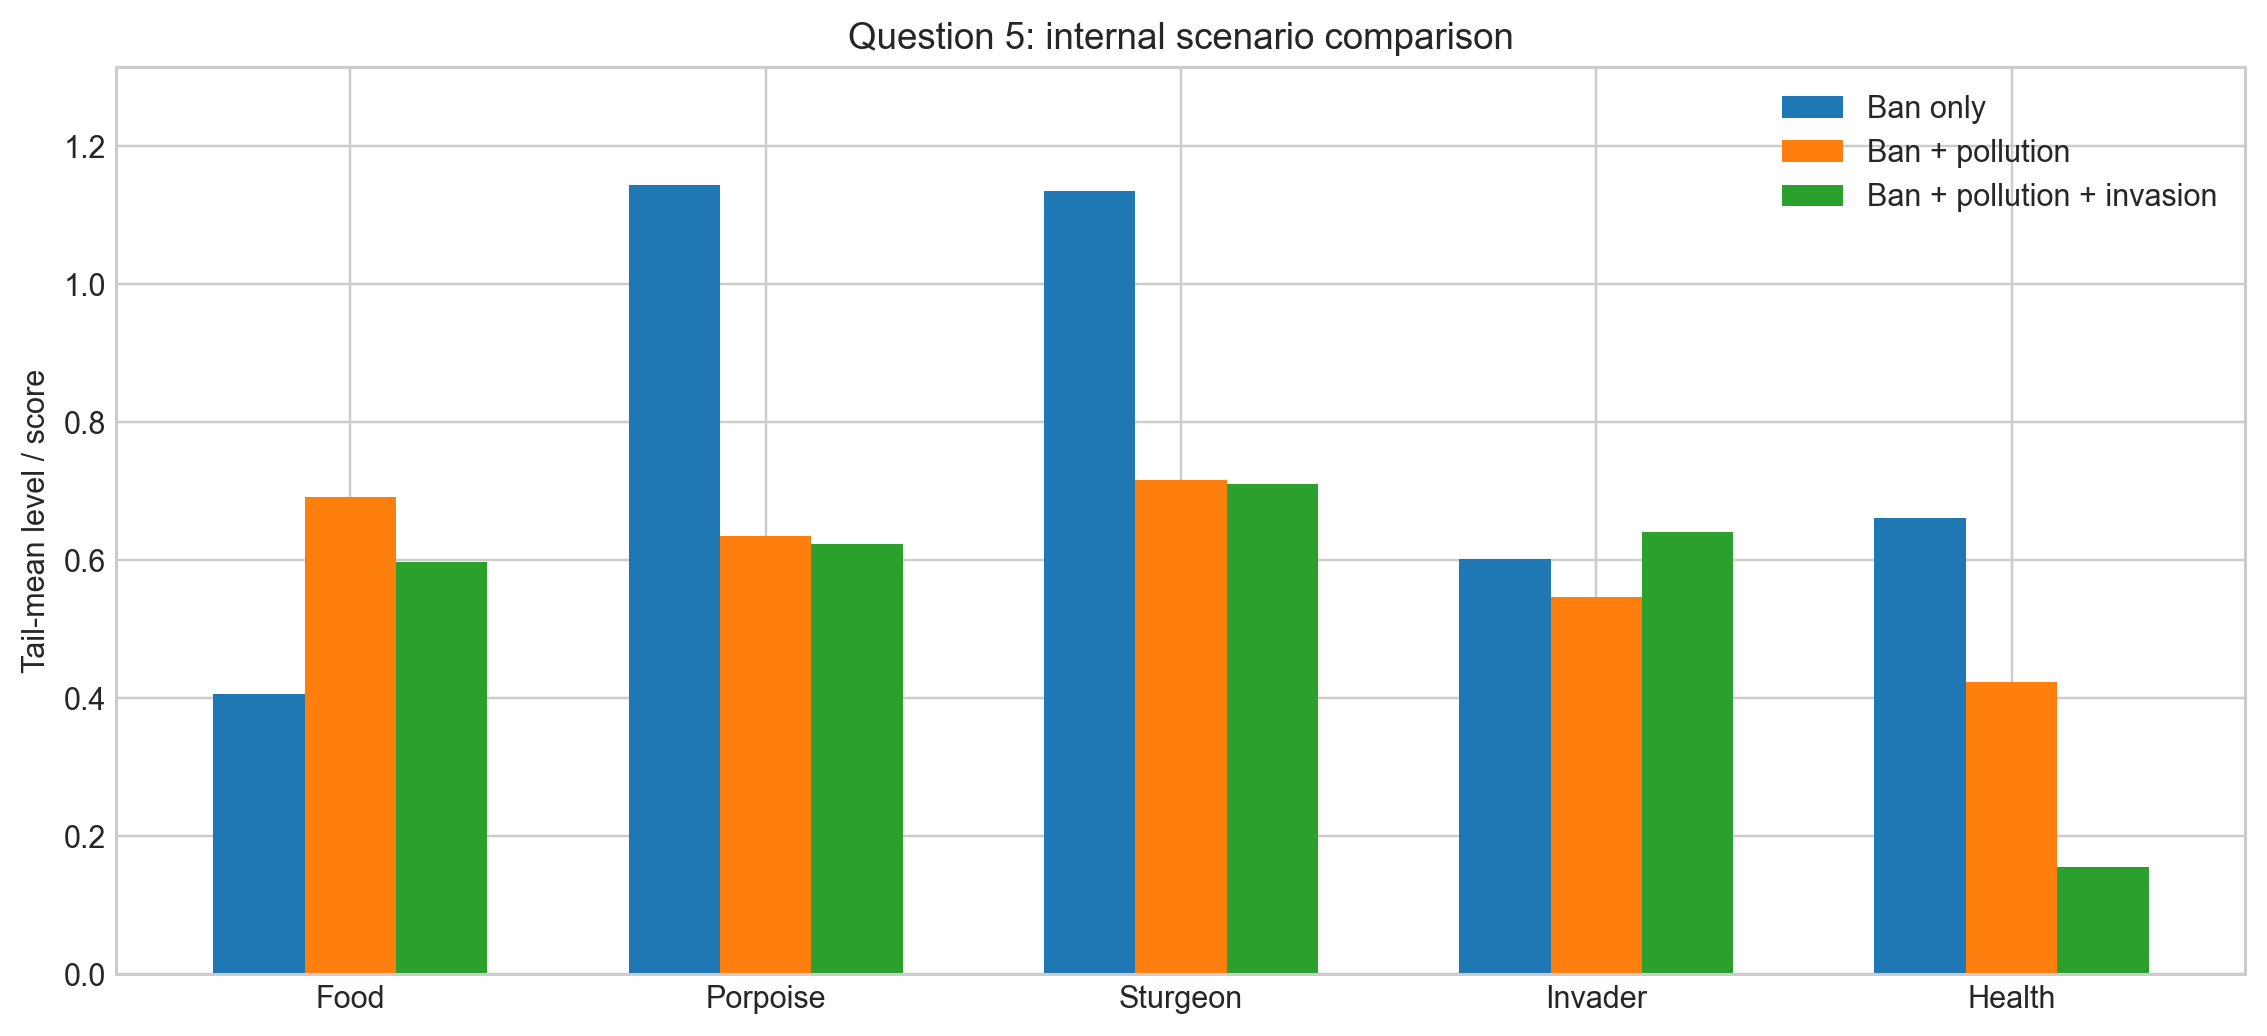
\includegraphics[width=0.88\textwidth]{fig05_q5_scenarios.png}
\caption{问题五的情景比较结果}
\label{fig:q5}
\end{figure}

\section{治理建议}
问题一中，四大家鱼恢复上升，水草、浮游动物和底栖饵料却可能下降；问题二中，江豚与长江鲟对通道和放流的响应又不一样。治理重点不能只停留在捕捞约束本身。后续监测最好同时列出四大家鱼总量、底层资源指标和食压指数；鱼道修复、产卵场连通及放流节律也不宜按同一办法处理。

更迫切的，是把污染治理和入侵控制往前提。问题五已经说明，污染情景的部分食源过程指标短时上升，珍稀物种终态和综合得分却在下降，所以局部过程变好并不等于系统整体好转。对入侵物种，可把鄱阳湖等支流湖泊作为高风险前沿，优先布设早期监测、拦截和清除，避免其沿食物网空档扩散。禁渔只是减轻了捕捞压力；如果水质治理、通道修复、放流优化和入侵防控接不上，恢复收益仍留不住。

\section{结论}
禁渔释放后，四大家鱼在模型中恢复到禁渔前约 1.8 倍，这是较早看到的正向结果；但同时看到，恢复主要还是积聚在消费者层。底层资源末值降至 0.204，食压指数持续上升，资源供给端并未随鱼群恢复同步转强。这里的末值和食压指数仅表示归一化压力水平，不直接对应全流域实测生物量结构。再往高营养级看，恢复收益还能继续传到长江江豚和长江鲟，只是这条路径并不稳：通道阻隔一加重，传导立刻变弱，而人工放流补上来的部分又更多落在长江鲟上。

承载力继续提高后，三级食物链不会一直维持规则振荡，而是会走向更复杂的长期波动。有限时间最大李雅普诺夫指数支持了这一方向，但还不足以给出唯一临界点；文中的 $K$ 也只表示归一化结构压力，而非长江某一实测承载量。污染和入侵则把另一层风险推了出来：食源过程量可能和珍稀物种终态开始分离。按我们的分析框架看，禁渔只是恢复链条的起点，后面能不能把收益留在系统内部，最终还得看水质、连通性、放流和入侵控制能不能跟上。

\section{模型评价与改进方向}

\subsection{单区食物网的解释边界}
单区食物网在流域平均尺度上能够同时容纳总量标定、局地对照和反事实比较。我们的标定结果下，2025 年四大家鱼总量为 1.805，CPUE 代理为 1.838；对 $gain\_scale$、$consumer\_scale$ 和 $F_0$ 做 $\pm10\%$ 扰动后，恢复方向和禁渔占优关系保持不变。进一步对资源增长、摄食耦合、转化效率和自然损失四组结构参数做 $\pm20\%$ 分组扰动，并在每组扰动后重新标定总量目标，CPUE 代理仍位于 1.824--1.840 区间。这一结构接近按食性配对的并联系统：四类资源分别与四类鱼直接耦合，用于识别哪一层首先承压，而资源间竞争与鱼类交叉摄食没有显式展开。

$\mathrm{CPUE}^*$ 权重仍带有经验成分，湖北段数据也具有局地网具口径。按现有设定，模型能够稳健支持的是“全流域平均恢复”和“局地恢复方向一致”，还不足以精确解释湖北段增幅。若要继续提高解释力，我们更关心的是补充标准化 CPUE 和连续河段监测，并在此基础上再引入横向竞争和交叉摄食，而不是只增加状态维度。

\subsection{珍稀物种响应的归因能力}
问题二把公报初值、通道阻隔、放流补偿和上游食源纳入同一响应框架后，连通性约束与工程补偿的异质作用得以区分。高阻隔会使江豚和长江鲟末值降至 0.901 和 0.856，无放流时长江鲟降至 0.519；配合 $\pm 20\%$ 参数敏感性结果看，江豚对自身摄食与转化参数更敏感，长江鲟则对放流强度更敏感。

这一部分的限制主要来自状态结构的简化。当前模型尚未展开分龄、繁殖季节和分阶段放流调度，也把江豚、长江鲟与入侵者对中层猎物的半饱和响应压缩在同一尺度上。按这一级别的简化，它更适合比较不同机制的相对强弱，而不直接外推为精细的长期种群预测。

\subsection{长期行为展示的适用范围}
Hastings-Powell 降维模型保留了“资源--消费者--捕食者”的最小反馈闭环，使承载力变化与轨道类型之间的关系可以在单一参数轴上比较。更关键的是，在这一层抽象里轨道形态确实会随 $K$ 改变。代表点 $K=1.795,2.665,4.800$ 的后期统计量表明，随着 $K$ 增大，波动幅度和峰间隔离散程度同步放大，复杂非线性波动并非单纯来自图像印象。

这一模型承担的是长期行为展示，而不是河段尺度的参数映射。$X_1,X_2,X_3$ 与前文功能群只保持营养级对应关系，不继承问题一的具体参数口径，因此它适合解释行为类型如何变化，而不适合反推具体河段的承载阈值；文中的 $K$ 只对应归一化结构压力水平。

\subsection{复杂化判据的稳健范围}
有限时间最大李雅普诺夫指数把轨道复杂化转化为可比较的数值判据。基准设置下，我们看到 $K=3.2186$ 附近出现局部由负转正的跨越，短时间窗内对相邻步长和局部初值仍可复现。

一旦将积分时长扩展至 150 和 200，正指数区间明显左移；75 组扩展测试中仅有 5 组保留 $\lambda_{\max}(3.20)<0<\lambda_{\max}(3.22)$。因此我们保留“复杂性随承载力提高而增强”的判断，而不把 3.2186 写成唯一阈值。更精细的分岔定位仍需更长积分时长、致密网格与分岔图交叉验证。

\subsection{综合评价的排序可信度}
问题五的综合评价只用于三种情景之间的相对比较。四个指标经正向化后，熵权、CRITIC、等权和 2000 次局部扰动都给出同一排序，其中“禁渔+污染+入侵”始终最差，复合压力的负向作用在当前比较框架下较为稳定。

综合分数不能替代单指标解释。食源、江豚和长江鲟仍对应不同层面的生态状态；若后续补入独立生态监测量并扩展污染、入侵强度梯度，排序结论的外推边界会得到明确界定。

\noindent 五个子问题共享同一条“恢复收益--上传导--长期复杂化--复合压力检验”的逻辑链。问题一和问题二给出收益出现的位置及其削弱机制，问题三和问题四刻画承载力提高后的行为变化方向，问题五则检验这部分收益在污染与入侵叠加下还能留下多少。我们统一时间口径、情景设定和上游输入，使不同模块之间能够互相传递信息而不至于脱节。

\noindent 按现有资料，模型目前更适用于方向性政策比较与机制解释。若后续补入连续河段监测、标准化 CPUE、珍稀物种年度调查以及污染分级资料，单区框架可以扩展为分段比较，长期动力学部分也能与实际营养级数据建立较为稳固的对应关系。

\section{参考文献}
\printbibliography[heading=none]

\appendix
\begin{center}
\heiti\zihao{4} 附\hspace{1pc}录
\end{center}
\section{问题一完整默认参数附表}
\begin{table}[htbp]
\centering
\caption{问题一完整默认参数附表}
\label{tab:q1_param_full}
\scriptsize
\setlength{\tabcolsep}{2.5pt}
\begin{tabularx}{0.93\textwidth}{>{\raggedright\arraybackslash}p{2.0cm} >{\raggedright\arraybackslash}p{1.6cm} >{\raggedright\arraybackslash}X >{\raggedright\arraybackslash}p{1.6cm}}
\toprule
参数 & 默认值 & 依据/说明 & 角色 \\
\midrule
\multicolumn{4}{l}{\textbf{资源增长与归一化基准}} \\
$r_1,r_2,r_3,r_4$ & \makecell[l]{$1.15,0.95,$\\$0.82,0.72$} & 归一化相对恢复速度排序，表示水草快于浮游植物、浮游植物快于浮游动物、浮游动物快于底栖饵料；用于维持营养级时间尺度分离。 & 时间尺度约束 \\
$K_1,K_2,K_3,K_4$ & $(1,1,1,1)$ & 统一固定为归一化承载上界，不对应河段实测承载量。 & 归一化基准 \\
\midrule
\multicolumn{4}{l}{\textbf{摄食耦合与饱和响应}} \\
$\alpha_1,\alpha_2,\alpha_3,\alpha_4$ & \makecell[l]{$1.22,0.92,$\\$0.84,0.76$} & Holling II 型摄食耦合强度，按 $j=1,2,3,4$ 分别对应水草--草鱼、浮游植物--鲢鱼、浮游动物--鳙鱼、底栖饵料--青鱼\cite{holling1959}。 & 结构耦合 \\
$h_1,h_2,h_3,h_4$ & \makecell[l]{$0.55,0.50,$\\$0.48,0.45$} & 饱和摄食拐点参数，使系统在归一化尺度下保持有界响应。 & 饱和约束 \\
\midrule
\multicolumn{4}{l}{\textbf{转化效率与自然损失}} \\
$e_1,e_2,e_3,e_4$ & \makecell[l]{$0.43,0.35,$\\$0.33,0.30$} & 归一化转化效率；沿“草鱼--水草、鲢鱼--浮游植物、鳙鱼--浮游动物、青鱼--底栖饵料”顺序设置为递减，避免消费者收益超过资源层可供给量级。 & 能量转化 \\
$m_1,m_2,m_3,m_4$ & \makecell[l]{$0.16,0.14,$\\$0.13,0.12$} & 归一化自然损失系数，与转化效率共同维持消费者层在禁渔和非禁渔情景下的数量级稳定。 & 背景损失 \\
\midrule
\multicolumn{4}{l}{\textbf{校准、反事实与场景控制}} \\
$consumer\_scale$ & $0.60$ & 固定缩放四大家鱼初值，保留既有物种占比，不由 2025 年观测标定估计。 & 初值规范化 \\
$gain\_scale$ & $1.45$ & 由 2025 年“四大家鱼恢复到禁渔前约 1.8 倍”这一总量约束单参数搜索得到。 & 唯一标定参数 \\
$F$（禁渔情景） & $0$ & 禁渔基线情景下共同捕捞压力取零；这里给出的是场景取值，而非新增独立参数。 & 基线政策设定 \\
$F_0$ & $0.25$ & 不禁渔反事实情景的固定共同捕捞压力，取自区间 $[0.10,0.40]$ 的中位值，不参与观测校准。 & 反事实对照 \\
$u$ & $0$ & 问题一中污染强度默认取零，避免与问题五的污染情景混用。 & 基线环境设定 \\
\midrule
\multicolumn{4}{l}{\textbf{观测代理与初值模板}} \\
$\mathrm{CPUE}^*$ 权重 & $(1,1,1,0.7)$ & 草鱼、鲢鱼、鳙鱼等权；青鱼因偏底栖、单网次可见性较低而保守下调。 & 捕获量代理 \\
$y_0^{\text{base}}$ & \makecell[l]{$(0.88,0.82,0.76,$\\$0.70,0.46,0.42,$\\$0.38,0.34)$} & 归一化初值模板，资源四维在前、鱼类四维在后；四类鱼在仿真前统一乘以 $consumer\_scale=0.60$。 & 状态初始化 \\
\bottomrule
\end{tabularx}
\normalsize
\end{table}
\section{完整 Python 源程序}
\lstinputlisting[language=Python,basicstyle=\scriptsize\ttfamily,breaklines=true]{../scripts/model_pipeline.py}

\end{document}
